\documentclass[10pt,wide]{mwart}
\usepackage{amsfonts}
\usepackage{amssymb}
\usepackage{graphicx}
\usepackage{svg}
\usepackage[utf8]{inputenc}
\usepackage{tikz}
\usepackage{tabularx}
%\usepackage{polski}
\usepackage[centertags]{amsmath}
\usepackage{amsthm}
\usepackage{newlfont}
\usepackage[polish]{babel}
\usepackage[T1]{fontenc}
\usepackage{listingsutf8}
\usepackage{xcolor}
\usepackage{url}
\newtheorem{lemat}{Lemat}
\newtheorem{tw}{Twierdzenie}
\newtheorem{przyklad}{Przykład}
\newtheorem{wn}{Wniosek}
\newtheorem{zad}{Zadanie}
\theoremstyle{definition}
\newtheorem{df}{Definicja}
\newtheorem{fc}{Fakt}
\newtheorem{uw}{Uwaga}
\newtheorem{szk}{Szkic dowodu}
\newtheorem{alg}{Algorytm}
\renewcommand*{\figurename}{Wykres}
\addto\captionspolish{\renewcommand{\figurename}{Wykres}}



%\textwidth 16cm
%\textheight 23.5cm
%\topmargin -1cm
%\oddsidemargin 0.5cm
%\evensidemargin 0.5cm
%\def\thefootnote{\arabic{footnote})}


\pagestyle{plain}
\begin{document}
\title{\textbf{Pracownia nr 2 z Analizy Numerycznej}\\
Sprawozdanie do zadania \textbf{P2.13}}
\author{Wiktor Garbarek}
\date{Wrocław, Listopad 2017}

\maketitle
 \thispagestyle{empty}
 \section{O interpolacji klasycznej, jej problemach i problemie interpolacji Hermite'a.}
 Interpolacja jest bardzo ważnym zagadnieniem w kontekście pomiarów czy upraszczania obliczeń. W wielu dziedzinach nauki, gdy wykonujemy jakieś pomiary,
 to niestety możemy to zrobić tylko i wyłącznie na zbiorze dyskretnym. Często jednak znając wyniki pomiarów czy też obliczeń w dwóch punktach
 (gdzie zrobiliśmy to relatywnie prosto) chcielibyśmy wiedzieć co się dzieje w przedziale pomiędzy (szczególnie, jeśli przewidujemy, że zjawisko jest ciągłe).
 Oprócz tego, jeśli przybliżamy jakąś funkcję w danym przedziale, to chcielibyśmy wiedzieć jak duży błąd towarzyszy temu przybliżeniu oraz, oczywiście, chcielibyśmy, by ten błąd był najmniejszy z możliwych.

 Wiemy doskonale, że klasyczna interpolacja dla nieodpowiedniego zestawu węzłów, abstrahując od postaci wielomianu interpolacyjnego i algorytmu wykorzystanego do znalezienia tego wielomianu, może dawać nam przybliżenia obarczone bardzo dużym błędem.
 Ponadto nie wykorzystuje ona wszystkich informacji, które możemy zmierzyć. Przykładowo w fizyce,
 próbując znaleźć funkcję przebytej drogi w określonym czasie, chcielibyśmy móc wykorzystać inne możliwe do zmierzenia wartości,
 takie jak prędkość i przyśpieszenie, które w naturalny sposób są odpowiednio pierwszą oraz drugą pochodną drogi po czasie.
 Takich fizycznych interpretacji pochodnej jest mnóstwo: m.in moc jest pochodną pracy po czasie, siła pochodną pędu po czasie, natężenie prądu elektrycznego pochodną ładunku po czasie etc.
 Oprócz tego możemy znaleźć też takie naturalne interpretacje pochodnej w chemii czy ekonomii.

 W takim razie wartym uwagi jest do rozpatrzenia problem znalezienia wielomianu interpolacyjnego, który oprócz przyjmowania określonych wartości przez ten wielomian pewnych punktach węzłowych, pochodna tego wielomianu przyjmowałaby także określone wartości pochodnych. Być może chcielibyśmy też, by kolejne pochodne również się zgadzały.
 Wielomian spełniający takie warunki nazywa się wielomianem interpolacyjnym Hermite'a\footnote{
 Uwaga: W problemie interpolacji Hermite'a wymagamy,
 żeby w jakimś węźle \(x_i\) określona została wartość funkcji i ewentualnie pierwsze \(m_i - 1\) wartości kolejnych pochodnych.
 Przykładowo, gdy chcemy, by w punkcie \(0\) nasz wielomian miał wartość 0, jego pochodna wartość \(1\), a druga pochodna wartość \(42\),
 jest problemem interpolacji Hermite'a, natomiast problem znalezienia wielomianu,
 którego druga pochodna w punkcie \(0\) dawała \(1\), a pierwsza pochodna w punkcie \(1 \) dawała \(0\) nie jest, wedle definicji podanej w tej pracy, problemem interpolacji Hermite'a. (Chociaż oczywiście nadal pozostaje ciekawym problemem do rozważenia)}
 \footnote{Warto zauważyć, że wiele angielskich źródeł, za wielomian interpolacyjny Hermite'a uznaje taki, dla którego wartości w węzłach, oraz wartości pierwszych pochodnych się zgadzają. Uogólnienie tutaj przedstawione często jest nazywane \emph{Osculating Interpolation}}
 \section{Interpolacja Hermite'a - strona teoretyczna.}
Gdy rozpatrujemy klasyczną interpolację, to istnienie wielomianu stopnia \(n\) przechodzącego przez \(n+1\) różnych punktów (zwanych też węzłami) jest w pewien sposób intuicyjnie oczywiste - wygląda jak rozwiązanie układu \(n \) równań ze względu na \(n\) zmiennych. Gdy chcemy być nieco bardziej formalni, to wystarczy zwrócić uwagę, że pewna macierz w tym układzie jest macierzą Vandermonde'a i jej wyznacznik jest niezerowy. Sprawa robi się mniej intuicyjna dla interpolacji Hermite'a - czy na pewno możemy dostać wielomian, który nie tylko w pewnych ustalonych punktach osiąga ustalone wartości, ale też pochodne w tych punktach osiągają ustalone wartości - i to nie tylko pierwsze pochodne, ale też drugie czy dalsze!
\begin{tw} (Jednoznaczność istnienia wielomianu Hermite'a)
Niech dane będą: liczba naturalna \(k\), liczby \(m_0, m_1, ..., m_k \in \mathbb{N}_+\), parami różne węzły \(x_0, x_1, ..., x_k\) oraz wielkości rzeczywiste \(y_i^{(i)}\) (\(i = 0,1,...,k; j = 0,1,...,m_k - 1\)). Przyjmijmy \(n := m_0 + m_1 + ... + m_k - 1 \). Wtedy istnieje dokładnie jeden wielomian \(H_n\) stopnia co najwyżej \(n\) spełniający następujące warunki:
\begin{equation}
H_n^{(j)}(x_i) = y_i^{(j)}
\end{equation}
dla \(i = 0, 1, ..., k\) oraz \(j = 0, 1, ..., m_k - 1\).
\begin{proof} (Istnienie rozwiązania)
  Okazuje się, że pomysł konstrukcji wielomianu Hermite'a oparty na postaci Newton'a klasycznego wielomianu interpolacyjnego, po pewnych uogólnieniach, jest matematycznie poprawny, tj. spełnione są równania (1).

Oznaczmy \(s_i := \sum_{j=0}^{i-1} m_i\), gdzie \(s_0 = 0\). Zauważmy, że każda liczba \(0 \leq l \leq n\) ma jednoznaczne przedstawienie w postaci \(l = s_i + j\),
 gdzie \(0 \leq i \leq k\) oraz \(0 \leq j \leq m_i - 1\).
Zdefiniujmy zatem wielomiany węzłowe następująco:
\begin{equation}
p_{s_i + j}(x) = (x-x_i)^j \cdot \Pi_{j=0}^{i-1}(x - x_j)^{m_j}
\end{equation}
Wtedy łatwo zauważyć, że \(p_{l}(x) = p_{s_i}(x)\cdot (x-x_i)^j \)
Przyjmijmy teraz dwa następujące oznaczenia
\begin{equation}
  P_l(x) = \sum_{q = 0}^{l-1}b_q\cdot p_q(x) \\
  Q_l(x) = \sum_{q = l+1}^{n}b_q\cdot p_q(x)
\end{equation}
Łatwo zauważyć następujący fakt
\begin{equation}
  H_n(x) = P_l(x) + b_l\cdot p_l(x) + Q_l(x) \text{   dla  } l=0,1,...,n \\
\end{equation}
gdzie przyjmujemy \(P_0 \equiv Q_n \equiv 0\)
W takim razie możemy zauważyć, że
\begin{equation}
  (x-x_i)^{j+1} | Q_l(x) \Rightarrow Q_l^{(j)}(x_i) \equiv 0
\end{equation}
\begin{equation}
H_n^{(j)} = P_l^{(j)}(x_i) + j!b_l\cdot p_{s_i}(x_i)
\end{equation}
\begin{equation}
b_l = \frac{y_i^{(j)} - P_l^{(j)}(x_i)}{j!\cdot p_{s_i}(x_i)}
\end{equation}
Łatwo teraz zauważyć, że rozwiązanie tego problemu istnieje - bowiem zaczynamy dla \(b_0 = y_0^{(0)}\),
a późniejsze współczynniki \(b_l\) obliczamy wykorzystując wcześniej skonstruowane współczynniki \(b_0,b_1,...b_{l-1}\).
\end{proof}
\begin{proof} (Jednoznaczność rozwiązania)
  Chcemy dowieść, że istnieje dokładnie jeden taki wielomian Hermite'a spełniający równania (1). Przeprowadzimy dowód analogiczny dla klasycznej interpolacji.
  Załóżmy zatem nie wprost, że istnieją dwa takie wielomiany \(H_n, W_n\), różne od siebie, które spełniają równania (1).
  Rozważając wielomian \(H_n - W_n\) możemy zauważyć, że jest on stopnia co najwyżej \(n\) oraz suma krotności jego pierwiastków wynosi \(n+1\).
  W takim razie, wielomian \(H_n - W_n \equiv 0\) na mocy zasadniczego twierdzenia algebry, a co za tym idzie \(H_n \equiv W_n\), co przeczy założeniu, że wielomiany są różne.
\end{proof}
\end{tw}

 \section{Algorytmy konstrukcji wielomianu Hermite'a.}
 \subsection{Postać Newtona}
 Dowód przedstawiony w poprzednim rozdziale dał nam jednocześnie dość wygodny i ogólny algorytm polegający na obliczaniu \(b_i\) jako ilorazów różnicowych.
 Ma on niestety swoje wady, o których powiemy za chwilę.
 Uwaga: indeksowanie tablicy w dwóch pierwszych algorytmach zaczynamy od \(1\), tj. jeśli wyciągamy element o indeksie \(1\) z tablicy \([a_0, a_1, a_2, ... a_k]\), to otrzymamy \(a_0\)
\begin{alg}
  \begin{verbatim}

      Wejście: [x_0, x_1, ..., x_k], [m_0, m_1, ..., m_k],
               [(y_0^0, y_0^1, ..., y_0^(m_0 - 1)), ...,
                                  (y_k^0, y_k^1, ..., y_k^(m_k - 1))]
      Wyjście: [b_0, b_1, ..., b_n]

      n := m_0 + m_1 + ... + m_k
      C_1 := dla i od 0 do k: m_i razy wstaw x_i do tablicy
      C_2 := dla i od 0 do k: m_i razy wstaw y_i^{(0)} do tablicy
      dla i od 3 do n+1:
        C_i = dla j od 1 do (n-(i-2)):
          jeśli C_1[j+i-2] - C_1[j] nie jest zerem
          to : wstaw (C_(i-1)[j+1] - C_(i-1)[j])/(C_1[j+i-2] - C_1[j])
          wpp: gdy w mianowniku występuje x_q to wstaw y_q^{i-2}/(i-2)!

      B := dla i od 2 do n+1: wstaw C_i[1]
      zwróć B
\end{verbatim}
\end{alg}
Łatwo zauważyć, że powyższy algorytm wykonuje \(O(n^2)\) obliczeń. Ponadto złożoność pamięciowa także wynosi \(O(n^2)\) (przechowujemy całą tablicę ilorazów różnicowych, których jest około \(\frac{n^2}{2}\))
Okazuje się, że złożoność pamięciową możemy zmniejszyć do \(O(n)\). Oczywiście musimy zachować kolumnę \(C_1\), w której trzymamy punkty węzłowe, zatem wszystkie operacje będziemy wykonywać na tablicy \(C_2\).
\begin{alg}
  \begin{verbatim}

      Wejście: [x_0, x_1, ..., x_k], [m_0, m_1, ..., m_k],
               [(y_0^0, y_0^1, ..., y_0^(m_0 - 1)), ...,
                                  (y_k^0, y_k^1, ..., y_k^(m_k - 1))]
      Wyjście: [b_0, b_1, ..., b_n]

      n := m_0 + m_1 + ... + m_k
      B_1 := dla i od 0 do k: m_i razy wstaw x_i do tablicy
      B := dla i od 0 do k: m_i razy wstaw y_i^{(0)} do tablicy
      dla i od 2 do n+1:
        dla j od n do i iterując o -1:
          jeśli B_1[j] - B_1[j-i+1] nie jest zerem
          to : B[j] := (B[j] - B[j-1])/(B_1[j] - B_1[j-i+1])
          wpp:
            znajdź takie q, że B_1[j] = x_q, wtedy
            B[j] := y_q^{i-1}/(i-1)!
      zwróć B
\end{verbatim}
\end{alg}
Gdzie operator postfiksowy ! to zwykła silnia.

Pojawiają się jednak problemy w tych obu algorytmach - obliczanie współczynników wielomianu w postaci Newtona nie jest numerycznie poprawne, a problem pojawia się przy dużej ilości węzłów.
Ogólnie, zdecydowanie lepszą pod względem własności numerycznych i poprawności jest postać barycentryczna wielomianu interpolacyjnego.
\subsection{Postać barycentryczna.}
Możemy za to wykorzystać postać barycentryczną ogólnego wielomianu Hermite'a zaproponowaną przez Wernera oraz Schneidera w \cite{CSWW}.
\begin{tw} (Schneider, Werner)
Postać barycentryczna wielomianu Hermite'a spełniającego warunki (1) ma następującą postać
\begin{equation}
  H(x) = \frac{\sum_{i=0}^{k}\sum_{j=0}^{m_i - 1}\frac{\alpha_{i,j}}{(x - x_i)^{j+1}}\sum_{l=0}^{j}\frac{y_i^{(l)}}{l!}(x-x_i)^l}{\sum_{i=0}^{k}\sum_{j=0}^{m_i - 1}\frac{\alpha_{i,j}}{(x - x_i)^{j+1}}}
\end{equation}.
Oznaczmy następująco przez \(\gamma_i(x) = \alpha_i(x)\Pi_{j=i+1}^{n}(x-x_j)^{m_j}\), gdzie \(\alpha_i(x) = \sum_{j=0}^{m_i - 1}\alpha_{i,m_i-j-1}(x-x_i)^j\)
oraz dla \(i=0,...,k\). Można dowieść, że \(\alpha_{i,m_i-j-1} = \gamma_i[(x_i)^{j+1}, (x_{i+1})^{m_{i+1}}, ..., (x_n)^{m_n}]\).
\end{tw}
Dowody tych zależności, jak i poprawności poniższego algorytmu wraz z szerszym wytłumaczeniem, można znaleźć w \cite{CSWW}.
\begin{alg}
  \begin{verbatim}

    Wejście: [x_0, x_1, ..., x_k], [m_0, m_1, ..., m_k],
             [(y_0^0, y_0^1, ..., y_0^(m_0 - 1)), ...,
                                (y_k^0, y_k^1, ..., y_k^(m_k - 1))]
    Wyjście: [a_0,0, ..., a_k,(m_k - 1)]

    dla i od 0 do k-1:
      dla d od i+1 do k:
        a := 1/(x_i - x_d)
        dla j od 0 do m_d - 1:
          B[i,0] = a * B[i,0]
          dla l od 1 do m_i - 1:
            B[i,l] = a*(B[i,l] - B[i,l-1])
          B[d,j] = B[d,j] - B[i, m_i - 1]
    dla i od 0 do k-1:
      dla l od 0 do m_i - 1:
        A[i, m_i - l - 1] = B[i,l]
    zwróć A
  \end{verbatim}
\end{alg}

\section{Błędy interpolacji Hermite'a oraz porównanie do interpolacji Newtona.}
Postaramy się sprawdzić jak wygląda błąd interpolacji Hermite'a, oraz porównać co jest lepsze -
mieć mniej węzłów i znać pochodną (interpolacja Hermite'a), czy mieć więcej węzłów, ale bez znajomości pochodnej (interpolacja Newtona).
Nasze testy oprzemy na dwóch klasach funkcji:
wielomianach stopni wyższych, niż zadana ilość węzłów
(w innym przypadku znajdowalibyśmy za każdym razem ten sam wielomian, co nie miałoby większego sensu),
oraz wielomianach trygonometrycznych, tj. funkcjach postaci \(f(x) = \sum_{i=0}^{n}(a_i\cos(ix) + b_i\sin(ix)\).
W tym drugim przypadku, bardzo prosto możemy znaleźć pochodną, bowiem zauważymy, że \(f'(x) = \sum_{i=1}^{n}(-\frac{a_i}{i})\sin(ix) + \frac{b_i}{i}\cos(ix)\)
Oprócz tego przetestujemy rzeczone interpolacje na paru funkcjach \(f(x) = e^{\pm x^2}\) oraz dla funkcji Rungego.
\subsection{Błędy interpolacji wielomianów wyższych stopni w węzłach równoodległych.}
Wszystkie wielomiany będziemy interpolować na przedziale \([-1,1]\). \\
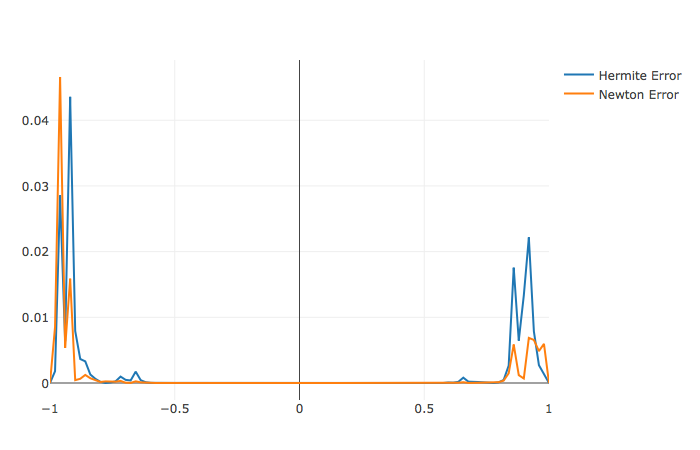
\includegraphics[scale=0.7]{polytesta.png}
\captionof{figure}{Wykres średniej arytmetycznej błędów względnych interpolacji dla 100 losowych wielomianów interpolowanych w 20 węzłach równoodległych (10 węzłów oraz pierwsze pochodne dla interpolacji Hermite'a).}
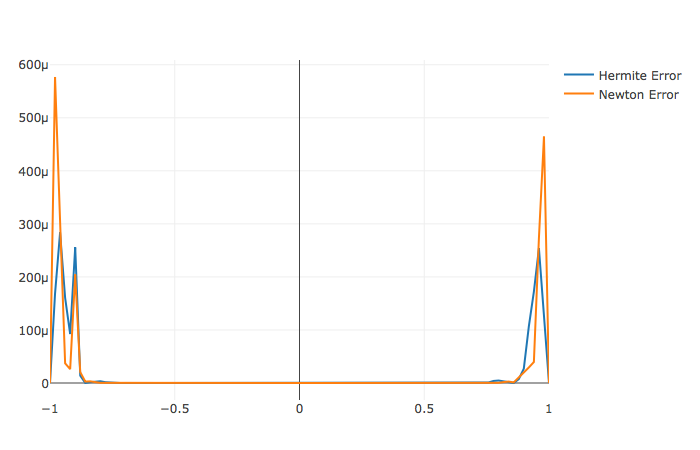
\includegraphics[scale=0.7]{polytestb.png}
\captionof{figure}{Wykres średniej arytmetycznej błędów względnych interpolacji dla 100 losowych wielomianów interpolowanych w 30 węzłach równoodległych (15 węzłów oraz pierwsze pochodne dla interpolacji Hermite'a).}
Możemy zauważyć, że interpolacja Hermite'a daje nieco lepsze przybliżenie wielomianu - pamiętajmy przy tym też, że mamy dwukrotnie mniej węzłów kosztem znajomości pochodnej, by stopień wielomianu interpolacyjnego został taki sam.
Redukuje ona też w lekkim stopniu efekt Rungego na krańcach przedziałów, ale niestety nie jest to duża poprawa.
\subsection{Błędy interpolacji wielomianów wyższych stopni w węzłach Czebyszewa.}
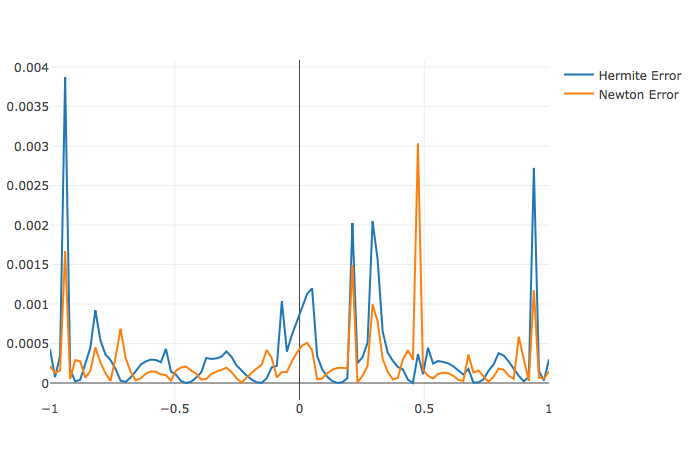
\includegraphics[scale=0.7]{polytestchebysheva.png}
\captionof{figure}{Wykres średniej arytmetycznej błędów względnych interpolacji dla 100 losowych wielomianów interpolowanych w 20 węzłach Czebyszewa (10 węzłów oraz pierwsze pochodne dla interpolacji Hermite'a).}
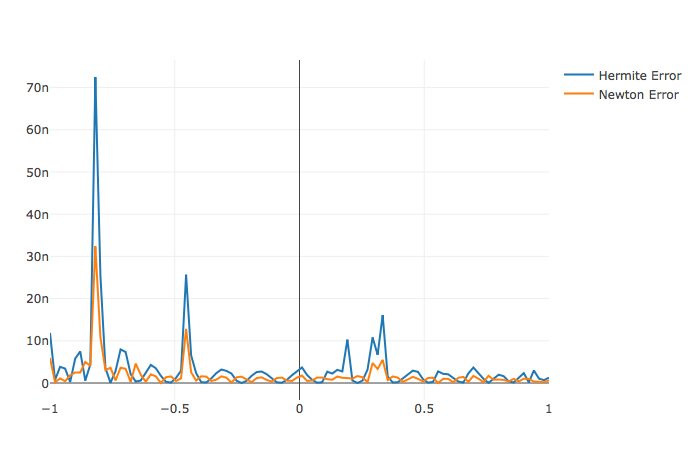
\includegraphics[scale=0.7]{polytestchebyshevb.png}
\captionof{figure}{Wykres średniej arytmetycznej błędów względnych interpolacji dla 100 losowych wielomianów interpolowanych w 30 węzłach Czebyszewa (15 węzłów oraz pierwsze pochodne dla interpolacji Hermite'a).}
Możemy zauważyć, że interpolacja Hermite'a w węzłach Czebyszewa nie daje lepszych efektów. \\
Błąd interpolacji jest jawnie zależny tylko od liczby węzłów, w przypadku interpolacji Hermite'a mamy dwa razy mniej węzłów niż w zwykłej interpolacji.
\subsection{Błędy interpolacji wielomianów trygonometrycznych w węzłach równoodległych.}
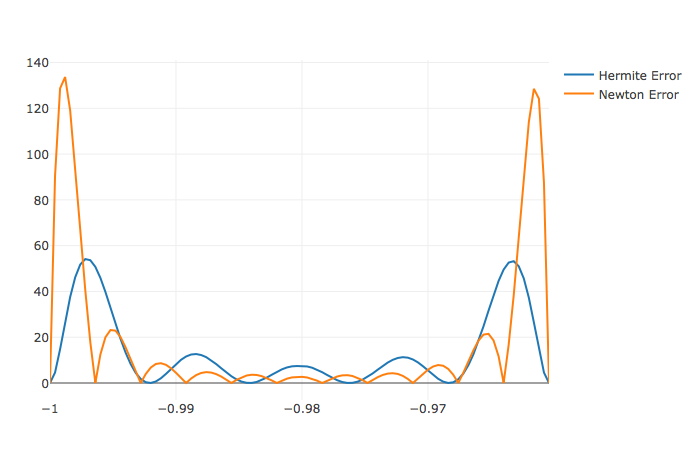
\includegraphics[scale=0.7]{trigtesterror.png}
\captionof{figure}{Wykres średniej arytmetycznej błędów bezwzględnych interpolacji dla 100 losowych wielomianów trygonometrycznych w 12 węzłach równoodległych (6 węzłów oraz pierwsze pochodne dla interpolacji Hermite'a).}
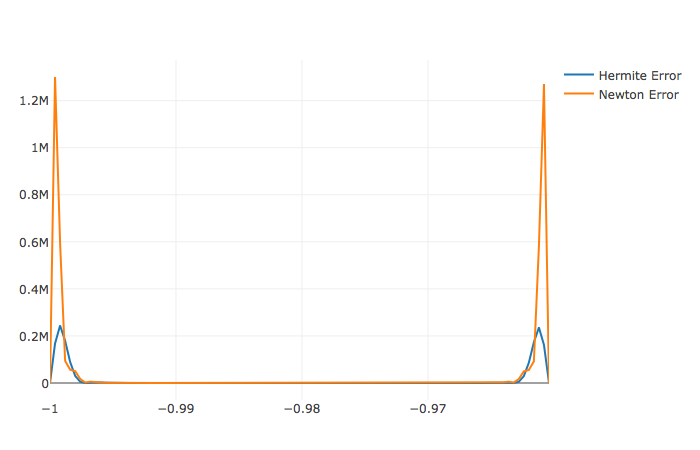
\includegraphics[scale=0.7]{trigtesterrorb.png}
\captionof{figure}{Wykres średniej arytmetycznej błędów bezwzględnych interpolacji dla 100 losowych wielomianów trygonometrycznych w 30 węzłach równoodległych (15 węzłów oraz pierwsze pochodne dla interpolacji Hermite'a).}
Możemy zauważyć, że interpolacja Hermite'a daje dość dobre efekty, bowiem przy dwa razy mniejszej ilości węzłów, ale przy znajomości wartości pierwszej pochodnej, znacznie redukujemy błędy interpolacji.
\subsection{Błędy interpolacji wielomianów trygonometrycznych w węzłach Czebyszewa.}
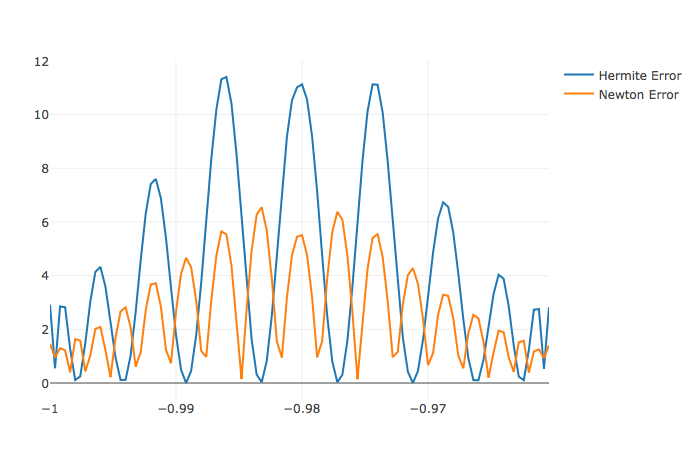
\includegraphics[scale=0.7]{trigtestchebysheva.png}
\captionof{figure}{Wykres średniej arytmetycznej błędów bezwzględnych interpolacji dla 100 losowych wielomianów trygonometrycznych w 20 węzłach Czebyszewa (10 węzłów oraz pierwsze pochodne dla interpolacji Hermite'a).}
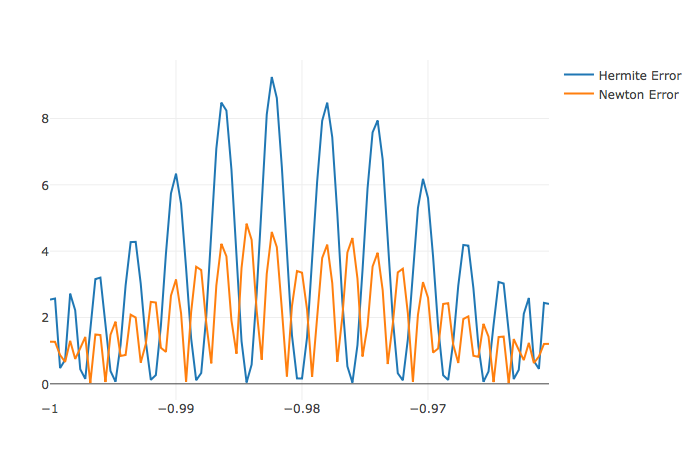
\includegraphics[scale=0.7]{trigtestchebyshevb.png}
\captionof{figure}{Wykres średniej arytmetycznej błędów bezwzględnych interpolacji dla 100 losowych wielomianów trygonometrycznych w 30 węzłach Czebyszewa (15 węzłów oraz pierwsze pochodne dla interpolacji Hermite'a).}
W tym przypadku jednak łatwo możemy zauważyć, że interpolacja Hermite'a nie daje praktycznie żadnych pozytywnych efektów. Wydaje się, że zdecydowanie lepsze jest dobranie kolejnych węzłów do interpolacji zamiast szukania
\subsection{Błędy interpolacji funkcji Rungego.}
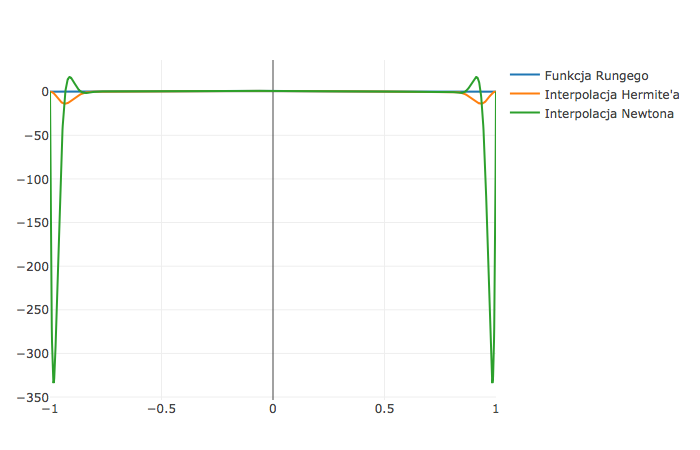
\includegraphics[scale=0.7]{rungeeffect.png}
\captionof{figure}{Wykres funkcji Rungego wraz z wielomianami interpolacyjnymi dla 30 węzłów (10 węzłów oraz wartości pierwszej i drugiej pochodnej dla interpolacji Hermite'a).}
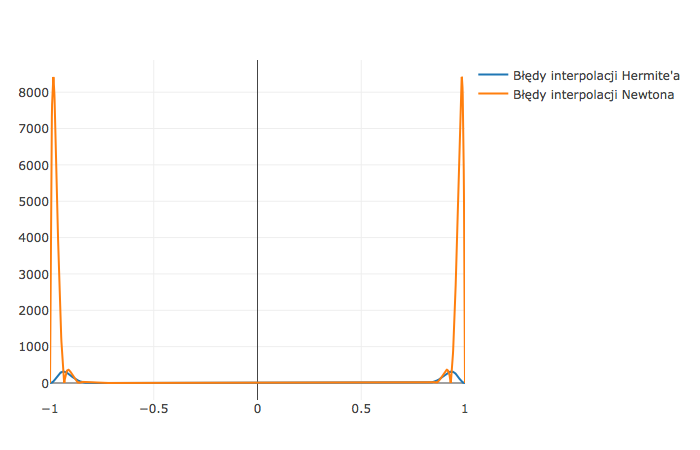
\includegraphics[scale=0.7]{rungeerror.png}
\captionof{figure}{Wykres funkcji błędów względnych interpolacji funkcji Rungego.}
Widzimy, że w przypadku interpolacja Hermite'a, mimo dużej poprawy względem zwykłej interpolacji, dalej jest dotknięta efektem Rungego.
\subsection{Błędy interpolacji funkcji \(e^{\pm x^2}\).}
Rozpatrzmy najpierw funkcję \(f(x) = e^{x^2}\).\\
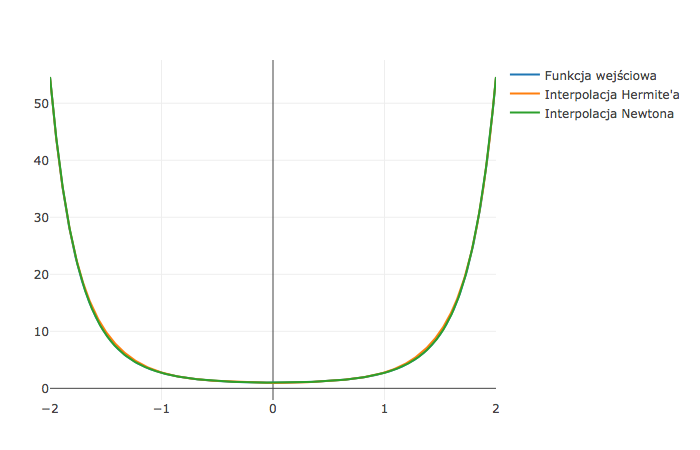
\includegraphics[scale=0.7]{einter.png}
\captionof{figure}{Wykres funkcji \(e^{x^2}\) oraz wieomianów interpolacyjnych dla 12 węzłów równoodległych (4 węzły oraz wartości pierwszej i drugiej pochodnej dla interpolacji Hermite'a).}
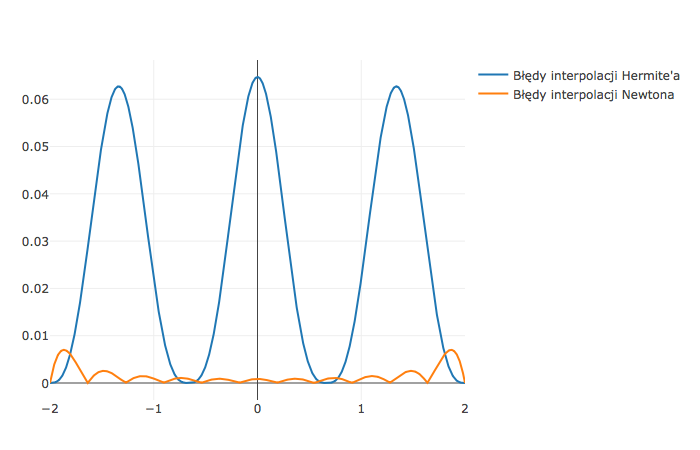
\includegraphics[scale=0.7]{eerror.png}
\captionof{figure}{Wykres funkcji błędów względnych interpolacji funkcji \(e^{x^2}\).}
Możemy dostrzec, że błąd interpolacji Hermite'a jest zdecydowanie większy, niż interpolacji klasycznej.
Mimo wiedzy, że \(e^{x^2}\) jest dość gładką funkcją, paradoksalnie znajomość pochodnej nie daje nam zbytniej przewagi nad klasyczną interpolacją.

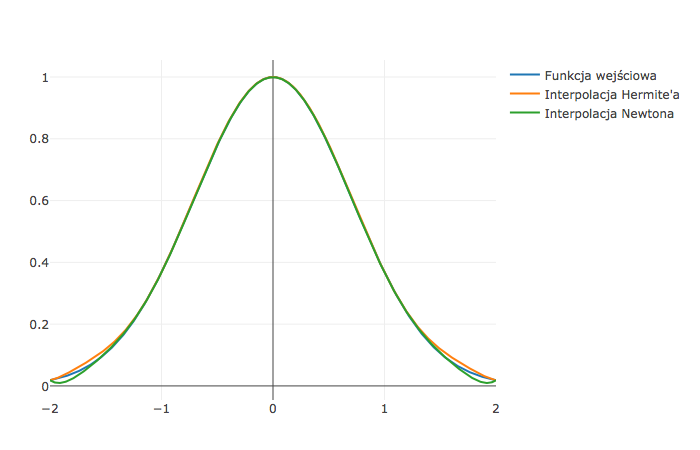
\includegraphics[scale=0.7]{eupinter.png}
\captionof{figure}{Wykres funkcji \(e^{-x^2}\) oraz wieomianów interpolacyjnych dla 12 węzłów równoodległych (4 węzły oraz wartości pierwszej i drugiej pochodnej dla interpolacji Hermite'a).}
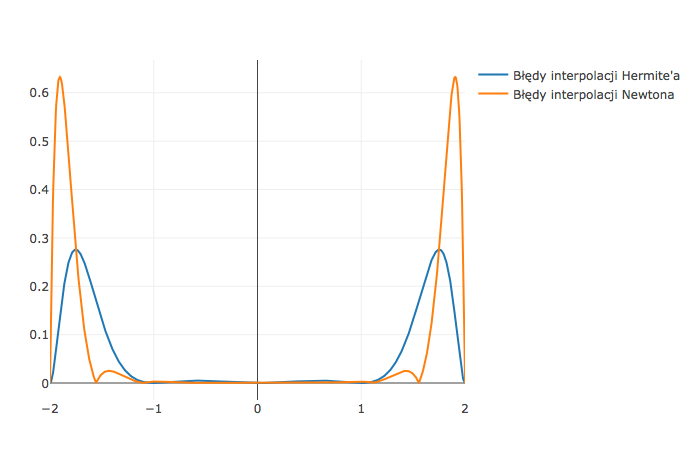
\includegraphics[scale=0.7]{euperror.png}
\captionof{figure}{Wykres funkcji błędów względnych interpolacji funkcji \(e^{-x^2}\).}

W tym przypadku jednak możemy dostrzec wyższość interpolacji Hermite'a.
Błędy interpolacji Hermite'a, mimo że są dość duże, to są zdecydowanie mniejsze niż błędy klasycznej interpolacji w trzy razy większej ilości punktów.

\section{Wnioski o użyteczności interpolacji Hermite'a.}
Na podstawie przeprowadzonych testów możemy zdecydować, że gdy zależy nam na jak najmniejszym błędzie interpolacji i nie martwimy się o wysoki stopień wielomianu,
to dodatkowa wiedza w postaci pochodnych da nam zdecydowanie lepsze wyniki.
Przede wszystkim każda znajomość pochodnej (bądź pochodnych) działa w pewien sposób jak dobranie dodatkowych węzłów do interpolacji klasycznej.
Jednakże, gdy zależy nam na minimalizacji stopnia wielomianu interpolacyjnego, to często lepszym rozwiązaniem będzie odpowiedni dobór węzłów, jeśli mamy taką możliwość.
Możemy też zauważyć, że na niekorzyść interpolacji Hermite'a działa występowanie podobnych problemów jak w klasycznej interpolacji (m. in. efektu Rungego).
Zdecydowanie lepszym i bardziej uniwersalnym wyjściem byłoby wykorzystanie funkcji sklejanych.


\begin{thebibliography}{9}
\itemsep10pt
\bibitem{JMJ} J. i M. Jankowscy, \emph{Przegląd metod i algorytmów numerycznych}, cz. 1, WNT, 1981.
\bibitem{CK} W. Cheney, D. Kincaid, \emph{Analiza numeryczna}, WNT, 2006.
\bibitem{WW} W. Werner, \emph{Polynomial interpolation: Lagrange versus Newton}, Mathematics of Computation 43, no. 167 (1984).
\bibitem{CSWW} C. Schneider, W. Werner \emph{Hermite interpolation: The barycentric approach}, Computing 46: 35, Springer, 1991.
\end{thebibliography}
\end{document}
